\documentclass[10pt]{article}
\usepackage[a4paper, margin=3.1cm]{geometry}
\usepackage[utf8]{inputenc}
\usepackage[german]{babel}
\usepackage{graphicx}
\usepackage{enumitem}
\usepackage{titlesec}
\usepackage{csquotes}
\usepackage{amsmath}

\titleformat{\section}
  {\normalfont\fontsize{12}{15}\bfseries}{\thesection.}{1em}{}

\title{\Large{\textbf{Bitcoin: Ein elektronisches Peer-to-Peer Geldsystem}}}
\author{Satoshi Nakamoto\\satoshin@gmx.com\\www.bitcoin.org}
\date{}

\begin{document}

	\maketitle
	
	\abstract{Eine reine Peer-to-Peer-Version eines elektronischen Geldsystems würde es ermöglichen, Online-Zahlungen von einer Partei direkt an eine andere zu senden ohne über ein Finanzinstitut zu gehen. Digitale Signaturen bilden einen Teil der Lösung, aber die Hauptvorteile gehen verloren, wenn weiterhin eine vertrauenswürdige dritte Partei notwendig ist, um Mehrfachausgaben zu verhindern. Wir schlagen eine Lösung für das Double-Spending-Problem (Problem der Mehrfachausgaben) vor, indem wir ein Peer-to-Peer-Netzwerk benutzen. Das Netzwerk gibt Transaktionen einen Zeitstempel, indem es diese in eine fortlaufende Kette von Hash-basierten Arbeitsbeweisen (Proof-of-Work) hasht. So erzeugt es eine Aufzeichnung, die nicht geändert werden kann ohne den Proof-of-Work neu zu erzeugen. Die längste Kette dient nicht nur als Nachweis für die Sequenz bezeugter Ereignisse, sondern auch als Beweis, dass sie vom größten Pool an CPU-Leistung stammt. Solange der Großteil der CPU-Leistung von Nodes kontrolliert wird, die nicht kooperieren, um das Netzwerk anzugreifen, werden diese die längste Kette generieren und schneller sein als die Angreifer. Das Netzwerk selbst erfordert nur eine Minimalstruktur. Nachrichten werden auf Best-Effort-Basis übertragen und die Nodes können das Netzwerk beliebig verlassen und wieder betreten, da sie die längste Proof-of-Work-Kette als Beweis darüber akzeptieren, was geschah, während sie weg waren.}
	
	\section{Einleitung}
	
	Es hat sich ergeben, dass der Handel im Internet inzwischen fast vollständig darauf beruht, dass Finanzinstitute als zu vertrauende dritte Parteien dienen, um elektronische Zahlungen zu verarbeiten. Während dieses System für die meisten Transaktionen ausreichend gut funktioniert, leidet es nach wie vor unter den Schwächen eines Modells, das auf Vertrauen beruht. Vollständig unumkehrbare Transaktionen sind nicht wirklich möglich, da Finanzinstitute es nicht vermeiden können, in Streitfällen zu vermitteln. Die Kosten der Vermittlung erhöhen die Kosten der Transaktion, was die Mindestgröße für machbare Transaktionen erhöht und die Möglichkeit kleiner Gelegenheitstransaktionen eliminiert. Ein größerer Schaden entsteht darüber hinaus durch den Wegfall der Möglichkeit, irreversible Zahlungen für irreversible Dienstleistungen zu tätigen. Durch die Option, Transaktionen rückgängig zu machen, erhöht sich das notwendige Vertrauen. Händler müssen ihren Kunden gegenüber misstrauisch sein und von ihnen mehr Informationen verlangen, als ansonsten notwendig wären. Ein bestimmtes Maß an Betrug wird als unvermeidbar akzeptiert. Diese Kosten und Zahlungsunsicherheiten können durch persönlichen Kontakt und die Verwendung einer physischen Währung vermieden werden, doch es existiert kein Mechanismus für die Leistung von Zahlungen über einen Kommunikationskanal ohne eine vertrauenswürdige Partei.

	Notwendig ist ein elektronisches Zahlungssystem, das auf kryptographischem Nachweis an Stelle von Vertrauen basiert und es zwei bereitwilligen Parteien ermöglicht, Transaktionen direkt untereinander durchzuführen ohne dass eine vertrauenswürdige dritte Partei benötigt wird. Transaktionen, bei denen es rechnerisch unmöglich ist, sie zu widerrufen, würden die Verkäufer vor Betrug schützen und standardisierte Treuhandmechanismen könnten auf einfache Weise implementiert werden, um die Käufer zu schützen. In diesem Paper schlagen wir eine Lösung für das Double-Spending-Problem vor, die unter Verwendung eines verteilten Peer-to-Peer-Zeitstempel-Servers einen rechnerischen Nachweis der chronologischen Reihenfolge der Transaktionen erzeugt. Das System ist sicher, solange die ehrlichen Nodes mehr CPU-Leistung kontrollieren als jede kooperierende Gruppe von angreifenden Nodes.
	
	\section{Transaktionen}
	Wir definieren eine elektronische Münze (Coin) als eine Kette digitaler Signaturen. Jeder Eigentümer überträgt den Coin auf den nächsten, indem er einen Hash der vorherigen Transaktion sowie den öffentlichen Schlüssel des nächsten Eigentümers digital signiert und dies an das Ende des Coins anhängt. Der Empfänger der Zahlung kann die Signaturen verifizieren, um die Kette der Eigentümer zu verifizieren.
	
	\begin{center}
		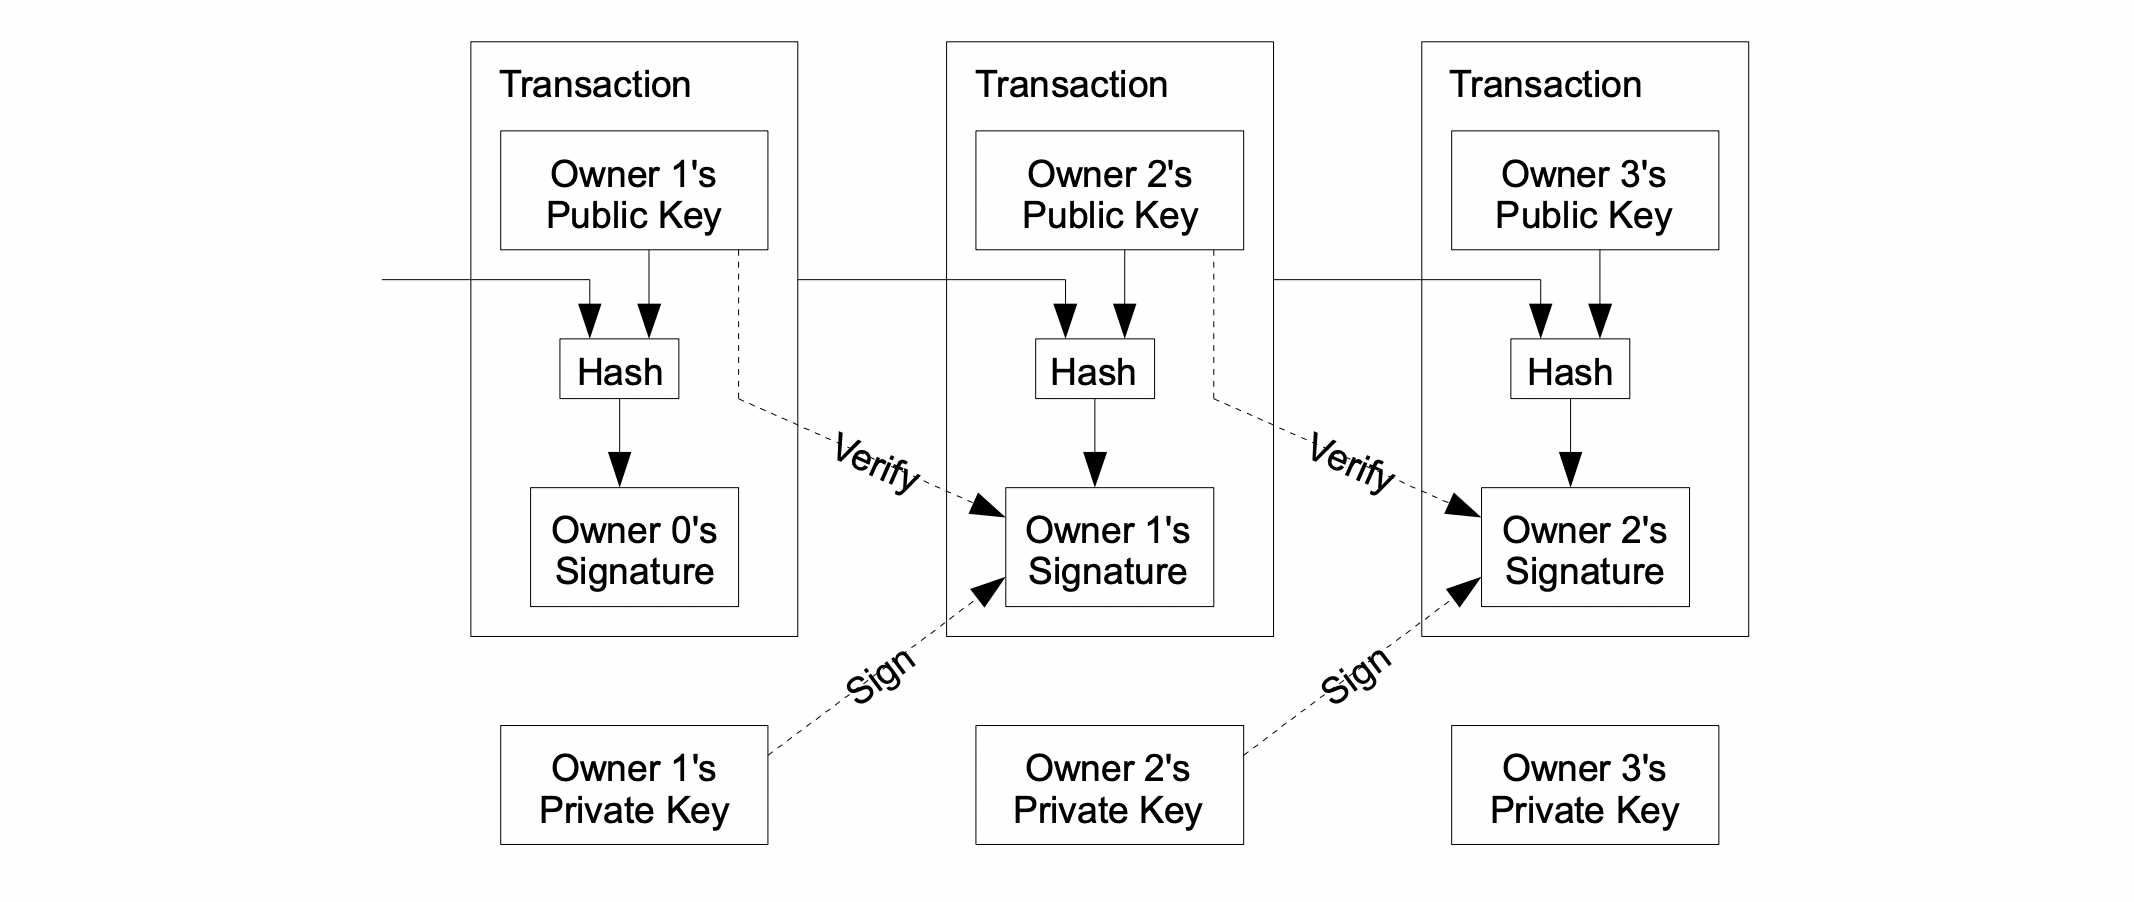
\includegraphics[scale=0.35]{pics/transactions.png}		
	\end{center}

	Das Problem ist natürlich, dass der Zahlungsempfänger nicht verifizieren kann, dass einer der Eigentümer den Coin nicht doppelt ausgegeben hat. Eine gebräuchliche Lösung ist, eine zentrale, vertrauenswürdige Instanz, oder Münzanstalt, einzuführen, die jede Transaktion auf Double Spending (Mehrfachausgabe) prüft. Nach jeder Transaktion muss der Coin an die Münzanstalt zurückgegeben werden, damit diese einen neuen Coin herausgibt und nur bei Coins, die direkt von der Münzanstalt ausgegeben wurden, kann darauf vertraut werden, dass sie nicht doppelt ausgegeben worden sind. Das Problem mit dieser Lösung ist, dass das Schicksal des gesamten Geldsystems von dem Unternehmen abhängt, das die Münzanstalt betreibt und dass jede Transaktion über dieses laufen muss, wie bei einer Bank.
	
	Wir brauchen eine Methode, um Gewissheit für den Zahlungsempfänger zu schaffen, dass die vorherigen Eigentümer keine früheren Transaktionen signiert haben. Für unsere Zwecke ist die erste Transaktion diejenige, die zählt, so dass wir uns keine Sorgen über spätere Versuche zur Mehrfachausgabe machen müssen. Die einzige Möglichkeit, die Abwesenheit einer Transaktion zu bestätigen, ist es, alle Transaktionen zu kennen. In dem auf einer Münzanstalt basierenden Modell kannte die Münzanstalt alle Transaktionen und konnte entscheiden, welche zuerst eingetroffen ist. Um dies ohne vertrauenswürdige Partei zu erreichen, müssen Transaktionen öffentlich gemacht werden [1] und wir benötigen ein System, mit dem sich die Teilnehmer auf einen einzigen Verlauf der Reihenfolge, in der sie eingetroffen sind, einigen. Der Zahlungsempfänger benötigt einen Nachweis, dass sich zum Zeitpunkt jeder Transaktion die Mehrheit der Knoten des Netzwerks einig sind, dass sie diese zuerst empfangen haben.

	\section{Zeitstempel-Server}
	
	\begin{center}
		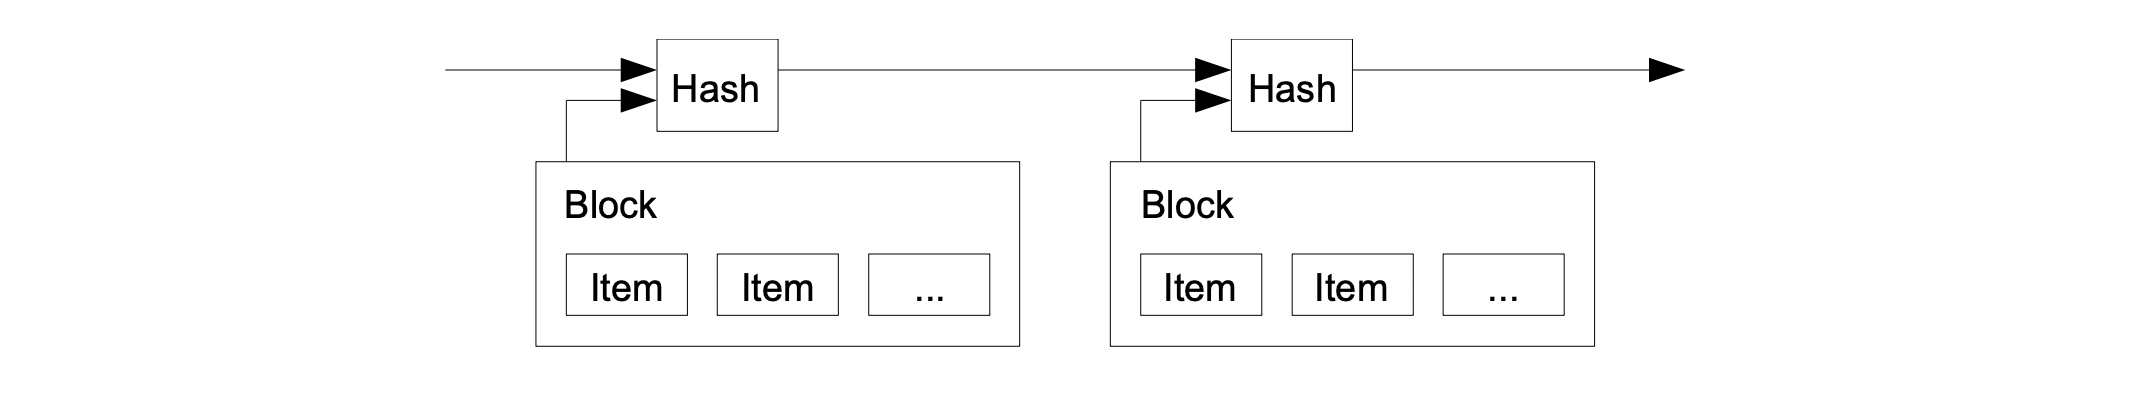
\includegraphics[scale=0.35]{pics/timestampserver.png}
	\end{center}

	\newpage
	
	\section{Proof-of-Work}
	
	Um einen verteilten Zeitstempel-Server auf Peer-to-Peer-Basis zu implementieren, müssen wir ein Proof-of-Work-System, ähnlich des Hashcash-Systems von Adam Back [6], anstatt der Zeitungen oder Usenet-Posts verwenden. Der Proof-of-Work beinhaltet die Suche nach einem Wert, bei dem, wenn er gehasht wird, etwa durch SHA-256, der Hash mit einer Anzahl von Nullbits beginnt. Die durchschnittlich erforderliche Arbeit ist exponentiell zu der Anzahl der erforderlichen Nullbits und kann durch die Ausführung eines einzelnen Hashs verifiziert werden.

	Für unser Zeitstempel-Netzwerk implementieren wir den Proof-of-Work, indem eine Nonce im Block solange ansteigt, bis ein Wert gefunden wird, der dem Hash des Blocks die erforderlichen Nullbits gibt. Nachdem die CPU genügend Arbeit aufgewendet hat, um den Proof-of-Work zu erfüllen, kann der Block nicht mehr geändert werden ohne dass die Arbeit erneut ausgeführt wird. Da spätere Blocks damit verkettet werden, würde die Arbeit zur Änderung des Blocks die Neuerstellung aller nachfolgenden Blocks beinhalten.
	
	\begin{center}
		
\includegraphics[scale=0.3]{pics/proofofwork.png}	
	\end{center}
	
	Der Proof-of-Work löst außerdem das Problem, bei Mehrheitsentscheidungen die Repräsentanten zu bestimmen. Wenn die Mehrheit auf einer Stimme je IP-Adresse basieren würde, könnte diese durch jeden unterwandert werden, der in der Lage ist, viele IPs zu reservieren. Proof-of-Work ist im Grunde eine Stimme pro CPU. Die Mehrheitsentscheidung wird durch die längste Kette repräsentiert, in die der größte Proof-of-Work Aufwand investiert wurde. Wenn eine Mehrheit der CPU-Leistung von ehrlichen Knoten kontrolliert wird, wird die ehrliche Kette am schnellsten wachsen und alle konkurrierenden Ketten abhängen. Um einen vergangenen Block zu ändern, müsste ein Angreifer den Proof-of-Work des Blocks sowie den aller nachfolgenden Blocks neu erzeugen und dann die ehrlichen Nodes einholen und überholen. Wir werden später demonstrieren, dass die Möglichkeit, dass ein langsamerer Angreifer aufholt, sich exponentiell verringert, je mehr nachfolgende Blöcke hinzugefügt werden.

	Um steigende Hardwareleistung und zeitlich schwankendes Interesse, einen arbeitenden Node zu betreiben, auszugleichen, wird die Proof-of-Work-Schwierigkeit durch einen gleitenden Mittelwert bestimmt, der eine durchschnittliche Anzahl von Blocks pro Stunde anpeilt. Wenn sie zu schnell generiert werden, steigt die Schwierigkeit.
	
	\section{Netzwerk}
	
	Die Schritte zum Betrieb des Netzwerks sind die Folgenden:
	
	\begin{enumerate}[label={\arabic*)}, topsep=0pt, itemsep=-1ex, partopsep=1ex, parsep=1ex]
		\item Neue Transaktionen werden an alle Knoten ausgestrahlt.
		\item Jeder Knoten sammelt die neuen Transaktionen in einem Block.
		\item Jeder Knoten arbeitet daran, einen schwierigen Proof-of-Work für seinen Block zu finden.
		\item Wenn ein Knoten einen Proof-of-Work findet, strahlt er den Block an alle Knoten aus.
		\item Die Knoten akzeptieren den Block nur, wenn alle Transaktionen darin gültig und nicht bereits ausgegeben sind.
		\item Die Knoten drücken ihre Akzeptanz des Blocks aus, indem sie daran arbeiten, den nächsten Block in der Kette zu erzeugen, wofür sie die Hash des akzeptierten Blocks als vorhergegangene Hash verwenden.
	\end{enumerate}
	
	Knoten gehen immer davon aus, dass die längste Kette die korrekte ist und arbeiten daran, diese zu verlängern. Wenn zwei Knoten gleichzeitig verschiedene Versionen des nächsten Blocks übertragen, könnten einige Nodes die eine oder die andere Version zuerst empfangen. In diesem Fall arbeiten sie an der ersten, die sie empfangen haben, speichern aber den anderen Zweig für den Fall, dass dieser länger wird. Der Gleichstand wird gebrochen, wenn der nächste Proof-of-Work gefunden wird und ein Zweig länger wird; die Nodes, die am anderen Zweig gearbeitet haben, werden dann auf den längeren umschalten.

	\newpage
	
	Die Ausstrahlung neuer Transaktionen muss nicht zwingend jeden Knoten erreichen. So lange sie viele Knoten erreichen, werden sie früher oder später in einem Block aufgenommen. Blockausstrahlungen sind auch tolerant gegenüber verlorenen Nachrichten. Wenn ein Knoten einen Block nicht empfängt, wird er diesen anfordern, sobald er den nächsten Block empfängt und erkennt, dass ihm einer fehlt.
	
	\section{Anreize}
	
	Durch Konvention ist die erste Transaktion in einem Block eine spezielle Transaktion, die einen neuen Coin schöpft, der dem Erzeuger des Blocks gehört. Dies gibt neuen Knoten einen Anreiz, das Netzwerk zu unterstützen und bietet einen Weg, Münzen erstmals in Umlauf zu bringen, da es keine zentrale Instanz gibt, die sie herausgibt. Das ständige Hinzufügen einer konstanten Anzahl neuer Coins ist analog zu Goldgräbern, die Ressourcen aufwenden, um mehr Gold in Umlauf zu bringen. In unserem Falle sind es CPU-Zeit und Elektrizität, die aufgewendet werden.

	Die Anreize können auch durch Transaktionsgebühren gefördert werden. Wenn der Ausgangswert der Transaktion geringer ist als ihr Eingangswert, entspricht der Unterschied einer Transaktionsgebühr, die dem Wert des Anreizes des Blocks hinzugefügt wird, der die Transaktion enthält. Wenn einmal eine vorherbestimmte Anzahl von Coins in Umlauf gebracht wurde, können die Anreize vollständig auf Transaktionsgebühren übergehen und so vollständig inflationsfrei sein.

	Die Anreize können helfen, Knoten zu motivieren, ehrlich zu bleiben. Wenn ein gieriger Angreifer in der Lage ist, mehr CPU-Leistung aufzubringen als alle ehrlichen Nodes, müsste er wählen, ob er diese Leistung verwendet, um Menschen zu betrügen, indem er seine Zahlungen zurück stiehlt, oder ob er sie nutzt, um neue Coins zu erzeugen. Er sollte es profitabler finden, sich an die Regeln zu halten — Regeln, die ihn mit mehr neuen Coins versorgen können als alle anderen zusammen — als dass er das System und damit die Gültigkeit seines eigenen Wohlstands untergräbt.

	\section{Speicherplatz zurück gewinnen}
	
	Sobald die letzte Transaktion eines Coins unter ausreichend Blöcken begraben ist, können die verbrauchten Transaktionen davor gelöscht werden, um Speicherplatz zu sparen. Um dies zu ermöglichen, ohne den Hash des Blocks zu brechen, werden die Transaktionen in einem Merkle-Tree \cite{merkle}\cite{massias}\cite{haber2} gehasht und lediglich die Root in die Hash des Blocks aufgenommen. Alte Blöcke können dann komprimiert werden, indem Zweige des Baumes gekappt werden. Die internen Hashes müssen nicht gespeichert werden.
	
	\begin{center}
		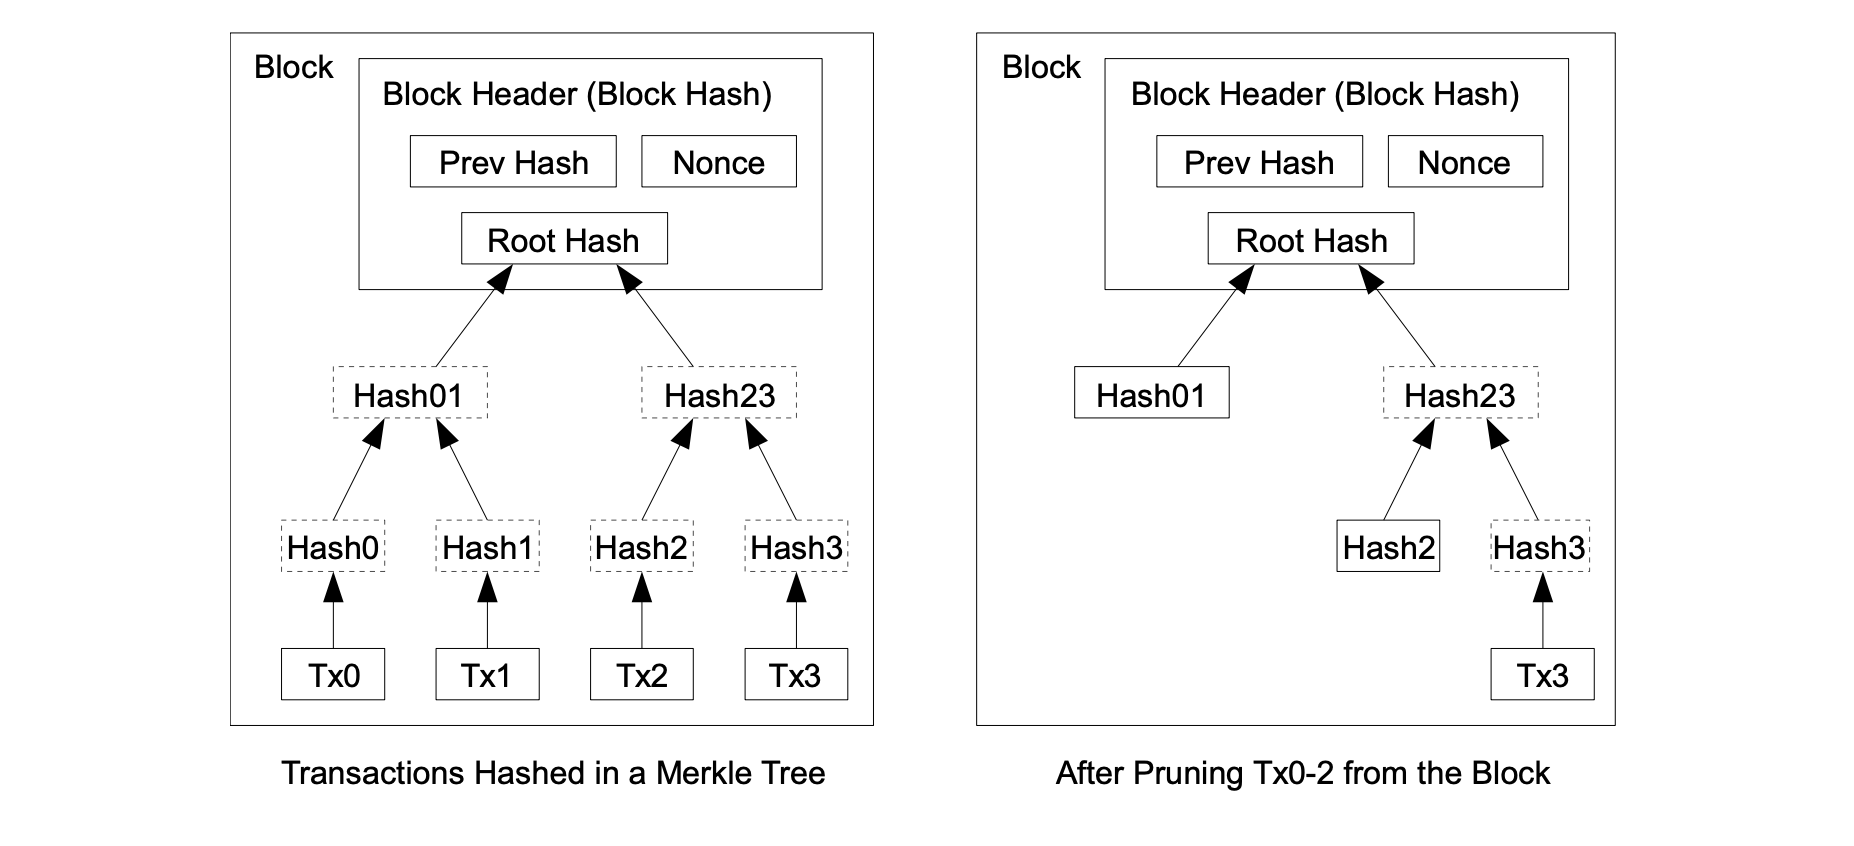
\includegraphics[scale=0.3]{pics/reclaimingdiskspace.png}
	\end{center}
	
	Ein Blockheader ohne Transaktionen benötigt etwa 80 Byte. Wenn wir davon ausgehen, dass Blöcke alle 10 Minuten generiert werden, entsprechen 80 Byte $* \;6 * 24 * 365 = 4,2$ MB pro Jahr. Mit Computersystemen, die im Jahr (Stand 2008) typischerweise mit 2 GB RAM verkauft werden und Moores Law, das aktuell ein Wachstum von 1,2 GB prognostiziert, sollte Speicherplatz kein Problem darstellen, selbst wenn die Blockheader im Speicher gehalten werden müssen.
	
	\section{Vereinfachte Zahlungsverifizierung}
	
	Es ist möglich Zahlungen zu verifizieren ohne einen kompletten Netzwerk-Node zu betreiben. Ein Nutzer muss lediglich eine Kopie der Blockheader der längsten Proof-of-Work-Kette aufbewahren, die er erhalten kann, indem er andere Netzwerk-Knoten solange abfragt, bis er überzeugt ist, dass er die längste Kette hat und den Merkle-Zweig beziehen, der die Transaktion mit dem Block verknüpft, durch den sie einen Zeitstempel erhalten hat. Er kann die Transaktion nicht selbst prüfen, aber indem er sie mit einer Stelle in der Kette verknüpft, kann er sehen, dass sie von einem Netzwerk-Node akzeptiert wurde und Blöcke, die danach angefügt wurden, bestätigen weiter, dass sie vom Netzwerk akzeptiert wurde.
	
	\begin{center}
		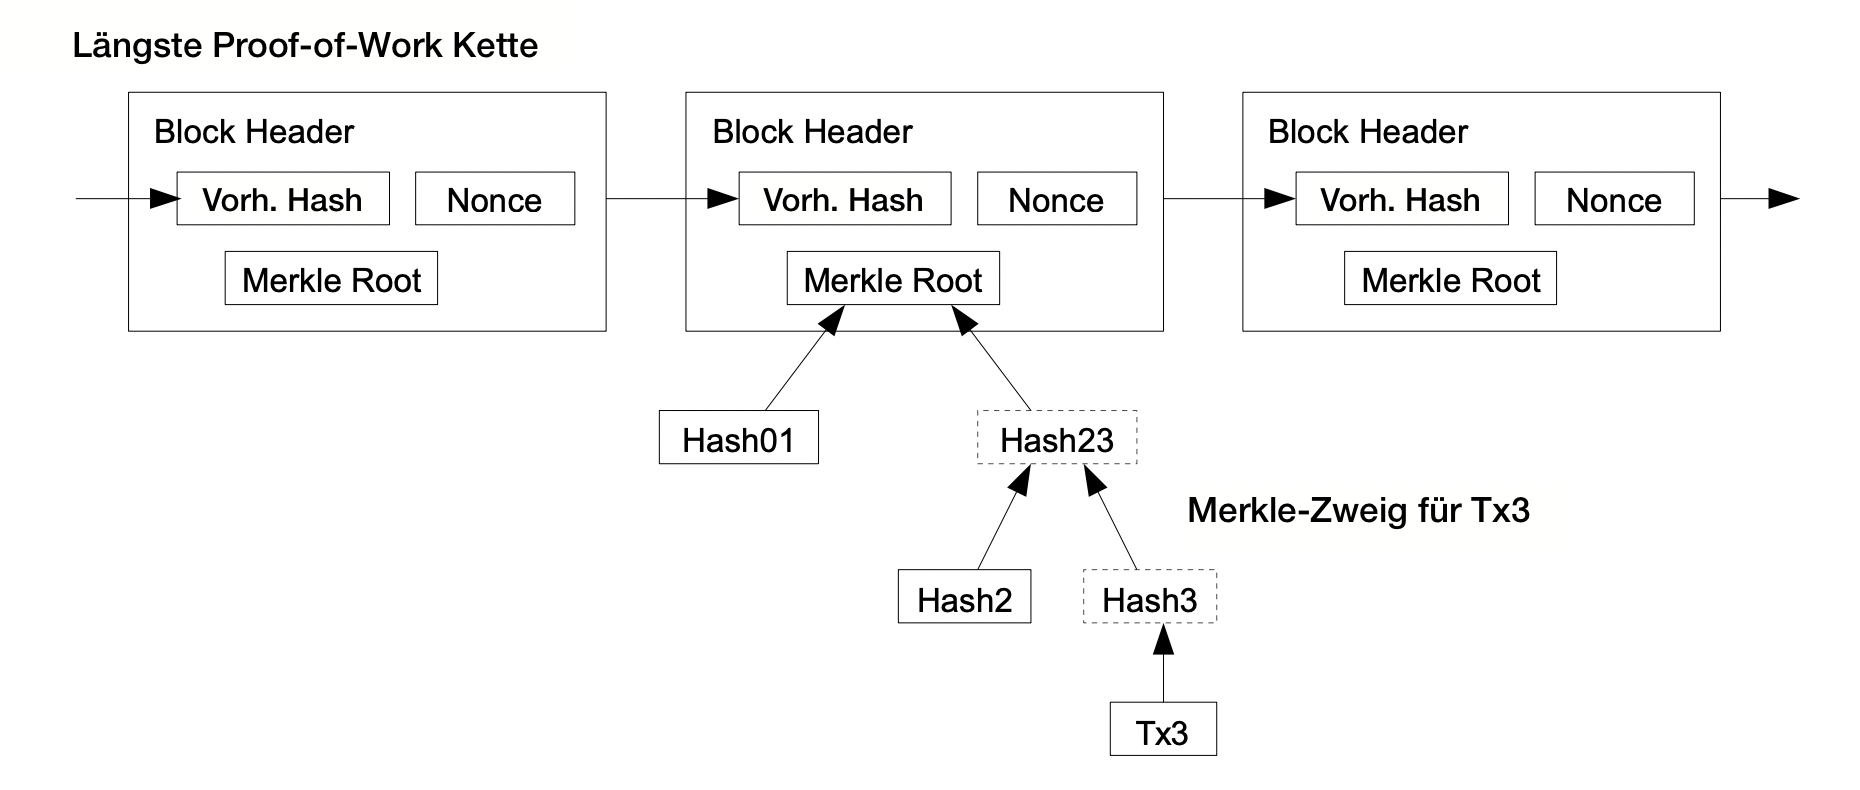
\includegraphics[scale=0.35]{pics/spv.png}
	\end{center}
	
	Als solche ist die Verifizierung zuverlässig, solange das Netzwerk von ehrlichen Nodes kontrolliert wird. Sie wird aber angreifbarer, wenn das Netzwerk von einem Angreifer überwältigt wird. Während Netzwerk-Knoten Transaktionen selbst verifizieren können, kann die vereinfachte Methode so lange durch einen Angreifer mit fingierten Transaktionen getäuscht werden, wie der Angreifer das Netzwerk dominieren kann. Eine Strategie, sich dagegen zu schützen, wäre es, Alarmsignale von Netzwerk-Nodes zu akzeptieren, wenn diese einen ungültigen Block erkennen, was die Software des Users veranlassen würde, den vollen Block und die vom Alarm betroffenen Transaktionen herunterzuladen, um die Inkonsistenz zu bestätigen. Unternehmen, die regelmäßige Zahlungen erhalten, werden dennoch ihre eigenen Nodes betreiben wollen, für eine unabhängigere Sicherheit und schnellere Verifizierung.

	\section{Zusammenführung und Aufteilung von Werten}
	
	Obgleich es möglich wäre, die Coins einzeln zu handhaben, wäre es unpraktisch, für jeden Cent in einem Transfer eine separate Transaktion durchzuführen. Damit Werte aufgeteilt und zusammengeführt werden können, enthalten Transaktionen mehrere Inputs und Outputs. Normalerweise gibt es entweder einen einzelnen Inputs von einer größeren vorausgegangenen Transaktion oder mehrere Inputs, die kleinere Beträge zusammenfassen und höchstens zwei Ausgänge: einer für die Zahlung und einer für die Rückgabe von Wechselgeld, falls notwendig, zurück an den Absender.
	
	\begin{center}
		
\includegraphics[scale=0.4]{pics/combineandsplit.png}
	\end{center}
	
	Es sollte erwähnt werden, dass eine Auffächerung, bei der eine Transaktion von mehreren Transaktionen abhängig ist und diese Transaktionen wiederum von vielen anderen abhängen, in diesem Fall kein Problem darstellt. Es besteht niemals die Notwendigkeit, eine vollständige Kopie eines Transaktionsverlaufs abzurufen.
	
	\newpage
	
	\section{Datenschutz}
	
	Das traditionelle Bankenmodell erreicht ein bestimmtes Datenschutzniveau, indem der Zugriff auf die Informationen auf die beteiligten Parteien und die vertrauenswürdige dritte Partei begrenzt wird. Die Notwendigkeit, alle Transaktionen zu veröffentlichen, schließt diese Methode aus, aber der Datenschutz kann dennoch aufrecht erhalten werden, indem der Informationsfluss an einer anderen Stelle unterbrochen wird: indem die öffentlichen Schlüssel anonym bleiben. Die Öffentlichkeit kann sehen, dass jemand einen Betrag an jemand anderen sendet, aber ohne Informationen, die die Transaktionen mit irgendjemandem verknüpfen. Das ist dem Level an Informationen ähnlich, das von Aktienbörsen veröffentlicht wird, bei dem die Zeit und die Größe der individuellen Handelsvorgänge, das “Tape”, veröffentlicht wird ohne dass dabei gesagt wird, wer die Parteien sind.
	
	\begin{center}
		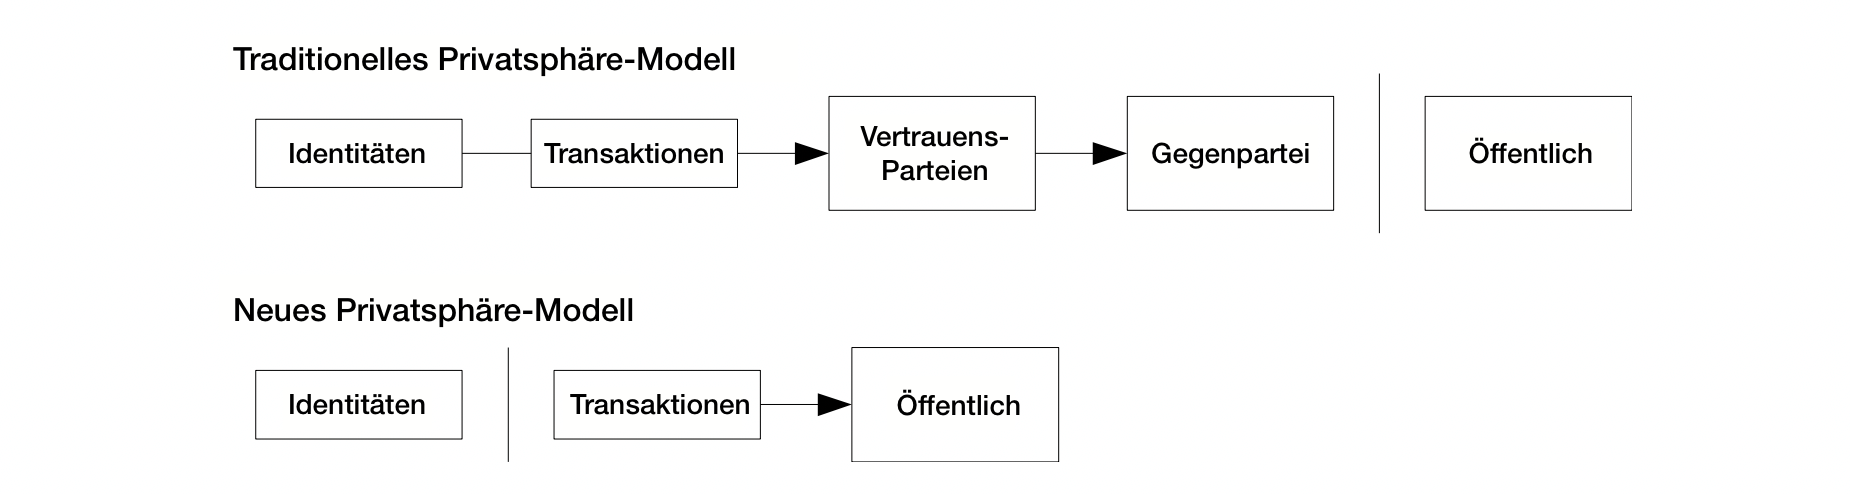
\includegraphics[scale=0.3]{pics/privacy.png}
	\end{center}
	
	Als zusätzliche Firewall sollte für jede Transaktion ein neues Schlüsselpaar verwendet werden, um zu vermeiden, dass die Schlüssel einem gemeinsamen Eigentümer zugeordnet werden können. Manche Verknüpfungen sind bei Transaktionen mit mehreren Eingängen noch immer unvermeidbar, weil diese notwendigerweise preisgeben, dass ihre Eingänge zum gleichen Eigentümer gehören. Das Risiko besteht darin, dass, wenn der Eigentümer eines Schlüssels bekanntgegeben wird, die Verknüpfung weitere Transaktionen offenlegen könnte, die zum gleichen Eigentümer gehört haben.
	
	\section{Berechnungen}
	
	Wir ziehen ein Szenario in Betracht, bei dem ein Angreifer versucht, eine alternative Kette schneller zu erzeugen als die ehrliche Kette. Selbst wenn dies gelingt, setzt es das System nicht willkürlichen Änderungen aus, wie zum Beispiel die Erzeugung von Wert aus dem Nichts oder das Nehmen von Geld, das dem Angreifer nicht gehört. Die Nodes werden keine ungültige Transaktion als Zahlung akzeptieren und die ehrlichen Nodes werden niemals einen Block akzeptieren, der eine solche enthält. Ein Angreifer kann lediglich versuchen, eine seiner eigenen Transaktionen zu verändern, um Geld zurück zu bekommen, das er vor kurzem ausgegeben hat.

	Das Rennen zwischen einer ehrlichen Kette und der Kette eines Angreifers kann als Binomischer Random Walk charakterisiert werden. Das Erfolgsereignis ist, dass die ehrliche Kette um einen Block erweitert wird, was deren Vorsprung um $+1$ erhöht und das Scheitern ist, dass die Kette des Angreifers um einen Block erweitert wird, was den Abstand um $-1$ reduziert.

	Die Wahrscheinlichkeit, dass ein Angreifer aus einem gegebenen Rückstand aufholt, ist analog zum Problem des “Ruin des Spielers”. Angenommen, ein Spieler mit unbegrenztem Kredit beginnt mit einem Rückstand und spielt potentiell eine unbegrenzte Anzahl von Partien, mit dem Ziel, die Gewinnschwelle zu erreichen. Wir können die Wahrscheinlichkeit, dass er jemals die Gewinnschwelle erreicht, oder dass ein Angreifer jemals eine ehrliche Kette einholt, wie folgt berechnen\cite{feller}:
	
	\vspace{2mm}
	\indent $p =$ Wahrscheinlichkeit, dass ein ehrlicher Node den nächsten Block findet\\
	\indent $q =$ Wahrscheinlichkeit, dass der Angreifer den nächsten Block findet\\
	\indent $q_z =$ Wahrscheinlichkeit, dass der Angreifer jemals den Rückstand von $z$ Blöcken aufholt
	

	\begin{flalign*}
\indent q_z = 
	\begin{cases}
		1, & \text{if} \ p \leq q \\
		(q/p)^z, & \text{if} \ p \geq q
	\end{cases}
\Biggl\} &&
	\end{flalign*}
	
	\newpage
	
	Unter unserer Annahme, dass $p > q$, fällt die Wahrscheinlichkeit exponentiell, wenn die Anzahl der Blocks, die der Angreifer aufholen muss, steigt. Wenn die Wahrscheinlichkeit gegen ihn ist und er nicht frühzeitig einen glücklichen Sprung vorwärts macht, werden seine Chancen verschwindend gering, wenn er weiter zurück fällt.

	Wir erörtern nun, wie lange der Empfänger einer neuen Transaktion warten muss, bis er ausreichend sicher ist, dass der Absender die Transaktion nicht mehr ändern kann. Wir nehmen an, dass der Absender ein Angreifer ist, der den Empfänger für eine Weile glauben lassen möchte, dass er bezahlt wurde und dann die Transaktion nach einiger Zeit verändert, so dass sie an ihn selbst zurückgezahlt wird. Der Empfänger wird alarmiert, wenn dies geschieht, aber der Absender hofft, dass es dann zu spät ist.

	Der Empfänger generiert ein neues Schlüsselpaar und gibt den Public Key kurz vor dem Signieren an den Sender. Dies verhindern, dass der Sender bereits im Voraus eine Kette von Blocks vorbereitet, indem er so lange daran arbeitet, bis er ausreichend Glück gehabt hat, um einen ausreichend großen Vorsprung zu haben und dann die Transaktion in diesem Moment ausführt. Wenn die Transaktion einmal abgeschickt wurde, beginnt der unehrliche Sender insgeheim mit der Arbeit an einer parallelen Kette, die eine geänderte Version seiner Transaktion enthält.

	Der Empfänger wartet, bis die Transaktion zu einem Block hinzugefügt wurde und z Blocks dahinter angefügt wurden. Er weiß nicht genau, welchen Fortschritt der Angreifer bereits gemacht hat, aber davon ausgehend, dass die ehrlichen Blocks die durchschnittliche Zeit pro Block benötigt haben, entspricht der potentielle Fortschritt des Angreifers einer Poisson-Verteilung mit dem erwarteten Wert:
	\begin{flalign*}
\indent \lambda = z \ \frac{q}{p} &&
	\end{flalign*}
	
	\noindent Um die Wahrscheinlichkeit zu berechnen, dass der Angreifer jetzt noch aufholen könnte, multiplizieren wir die Poisson-Dichte für jede Summe des Fortschritts, den er gemacht haben könnte, mit der Wahrscheinlichkeit, dass er von diesem Punkt an aufholen könnte:
	
	\begin{flalign*}
\indent \sum_{k = 0}^{\infty} \frac{\lambda^k e^{-\lambda}}{k!} \cdot 
	\begin{cases}
		(q/p)^{(z-k)}, & \text{if} \ k \leq z\\
		1, & \text{if} \ k > z
	\end{cases}
\Biggl\}&&
	\end{flalign*}
	
	\noindent Wir stellen die Formel um, um zu vermeiden, dass die unendlichen Nachkommastellen der Verteilung addiert werden…
	
	\begin{flalign*}
\indent 1 - \sum_{k = 0}^{z} \frac{\lambda^k e^{-\lambda}}{k!} (1- (p/q)^{(z-k)})&&
	\end{flalign*}
	
	\noindent Übersetzen in C Code...
	
	\begin{verbatim}
#include <math.h>
double AttackerSuccessProbability(double q, int z)
{
    double p = 1.0 - q;
    double lambda = z * (q / p);
    double sum = 1.0;
    int i, k;
    for (k = 0; k <= z; k++)
    {
        double poisson = exp(-lambda);
        for (i = 1; i <= k; i++)
            poisson *= lambda / i;
        sum -= poisson * (1 - pow(q / p, z - k));
    }
    return sum;
}
	\end{verbatim}
	
	\newpage
	
	\noindent Wenn wir einige Ergebnisse durchlaufen lassen, können wir erkennen wie die Wahrscheinlichkeit exponentiell mit $z$ abfällt.
	
	\begin{verbatim}
q=0.1
z=0 P=1.0000000
z=1 P=0.2045873
z=2 P=0.0509779
z=3 P=0.0131722
z=4 P=0.0034552
z=5 P=0.0009137
z=6 P=0.0002428
z=7 P=0.0000647
z=8 P=0.0000173
z=9 P=0.0000046
z=10 P=0.0000012

q=0.3
z=0 P=1.0000000
z=5 P=0.1773523
z=10 P=0.0416605
z=15 P=0.0101008
z=20 P=0.0024804
z=25 P=0.0006132
z=30 P=0.0001522
z=35 P=0.0000379
z=40 P=0.0000095
z=45 P=0.0000024
z=50 P=0.0000006
	\end{verbatim}
	
	\noindent Auflösung für P kleiner als 0,1\% …
	
	\begin{verbatim}
P < 0.001
q=0.10 z=5
q=0.15 z=8
q=0.20 z=11
q=0.25 z=15
q=0.30 z=24
q=0.35 z=41
q=0.40 z=89
q=0.45 z=340
	\end{verbatim}
	
	\section{Fazit}
	
	Wir haben ein System für elektronische Transaktionen vorgeschlagen ohne uns auf Vertrauen stützen zu müssen. Wir sind vom üblichen System von aus digitalen Signaturen erstellten Coins ausgegangen, das eine starke Kontrolle über die Eigentümerschaft bietet, aber unvollständig ist ohne eine Methode, um Doppelausgaben zu verhindern. Um dieses Problem zu lösen, haben wir ein Peer-to-Peer-Netzwerk vorgeschlagen, das Arbeitsbeweise benutzt, um eine öffentliche Historie von Transaktionen aufzuzeichnen, die für einen Angreifer unmöglich veränderbar sind, solange ehrliche Nodes die Mehrheit der CPU-Leistung kontrollieren. Das Netzwerk ist in seiner unstrukturierten Einfachheit robust. Die Nodes arbeiten alle zur gleichen Zeit mit nur wenig Koordination. Sie müssen nicht identifiziert werden, da die Nachrichten nicht zu einer bestimmten Stelle geleitet werden und nur auf Basis der besten Bemühungen ausgeliefert werden müssen. Nodes können das Netzwerk nach Belieben verlassen bzw. diesem beitreten und den Proof-of-Work als Nachweis dafür akzeptieren, was während ihrer Abwesenheit geschehen ist. Sie stimmen mit ihrer CPU-Leistung ab, drücken ihre Akzeptanz von zulässigen Blocks dadurch aus, dass sie an deren Erweiterung arbeiten und weisen ungültige Blocks dadurch ab, dass sie sich weigern, an diesen weiter zu arbeiten. Alle erforderlichen Regeln und Anreize können mit Hilfe dieses Konsensmechanismus durchgesetzt werden.
	
	\newpage
	
	\begin{thebibliography}{8}
	
		\bibitem{dai}W. Dai, \enquote{b-money}, http://www.weidai.com/bmoney.txt, 1998.
		
		\bibitem{massias}H. Massias, X.S. Avila, and J.-J. Quisquater, \enquote{Design of a secure timestamping service with minimal trust requirements}, In \emph{20th Symposium on Information Theory in the Benelux}, May 1999.
		
		\bibitem{haber}S. Haber, W.S. Stornetta, \enquote{How to time-stamp a digital document}, In \emph{Journal of Cryptology}, vol 3, no 2, pages 99-111, 1991.
		
		\bibitem{bayer}D. Bayer, S. Haber, W.S. Stornetta, \enquote{Improving the efficiency and reliability of digital time-stamping}, In \emph{Sequences II: Methods in Communication, Security and Computer Science}, pages 329-334, 1993.
		
		\bibitem{haber2}S. Haber, W.S. Stornetta, \enquote{Secure names for bit-strings}, In \emph{Proceedings of the 4th ACM Conference on Computer and Communications Security}, pages 28-35, April 1997.
		
		\bibitem{back}A. Back, \enquote{Hashcash - a denial of service counter-measure}, \\http://www.hashcash.org/papers/hashcash.pdf, 2002.
		
		\bibitem{merkle}R.C. Merkle, \enquote{Protocols for public key cryptosystems}, In \emph{Proc. 1980 Symposium on Security and Privacy}, IEEE Computer Society, pages 122-133, April 1980.
		
		\bibitem{feller}W. Feller, \enquote{An introduction to probability theory and its applications}, 1957.
	\end{thebibliography}
	
	\vfill
	\begin{center}
		\scriptsize{Deutsche Übersetzung: Blocktrainer.de\\ \smallskip \LaTeX: Sebastian Sutter}
	\end{center}
\end{document}





















